\documentclass{beamer}
\usepackage[english]{babel}
\usepackage[utf8]{inputenc}
\usepackage{hyperref}
\definecolor{links}{HTML}{2A1B81}
\hypersetup{colorlinks,linkcolor=,urlcolor=links}
\usetheme{default}
\usecolortheme{beaver}
\title[Ten Rules for Open Development of Scientific Software]{Article: Ten Simple Rules for the Open Development of Scientific Software}
\author{Brynjar Smári Bjarnason}
\institute{KTH -- School of Computer Science and Communication\\
\tiny \href{http://www.ploscompbiol.org/article/info\%3Adoi\%2F10.1371\%2Fjournal.pcbi.1002802}{link to article} \normalsize }
\date{\today}
\begin{document}

\section{Introduction}

\begin{frame}
\titlepage
\end{frame}

\subsection{Introduction}
\begin{frame}{Introduction}
Open source software
\begin{itemize}
\item Among the most cited publication
\item High impact
\item Wide user base
\end{itemize}
Pojects such as
\begin{itemize}
\item \href{http://wiki.galaxyproject.org/Admin/License}{Galaxy}, Bio[\href{http://www.biopython.org/DIST/LICENSE}{Python} \textbar \href{http://www.bioperl.org/wiki/Perl_Artistic_License}{Perl} \textbar \dots], 
	\href{http://emboss.sourceforge.net/licence/}{EMBOSS}, \href{http://metavelvet.dna.bio.keio.ac.jp/}{MetaVelvet}, \href{http://www.taverna.org.uk/about/legal-stuff/taverna-licence/}{Taverna}, 
	\href{http://docs.python.org/3.3/license.html}{Python}, \href{http://www.r-project.org/Licenses/}{R}
\end{itemize}
\end{frame}
\section{Ten rules}
\begin{frame}{Ten rules}
\begin{enumerate}
\item Don't reinvent the wheel
\item Code well
\item Be your own user
\item Be transparent
\item Be simple
\item Don't be a perfectionist
\item Nurture and grow your community
\item Promote your project
\item Find sponsors
\item Science counts
\end{enumerate}
\end{frame}
\subsection{Don't reinvent the wheel}

\begin{frame}{Don't reinvent the wheel}

\begin{itemize}
\item Many algorithms and methods already implemented
\begin{itemize}
\item Check if your problem has been solved
\item Break down your problem and check if parts have been solved
\end{itemize}
\item If an open source project could be fitted to your problem, it might be a good idea to collaborate rather than re-implement.
\item You can estimate if collaboration is appropriate by evaluating the source 
\end{itemize}
\end{frame}

\subsection{Code well}

\begin{frame}{Code well}
\begin{itemize}
\item Know the basics of software development
\item Read code
\item Improve open source code and send patches
\pause
\item READ CODE
\item You learn a lot of tips and tricks by reading code, \href{https://github.com/biopython/biopython}{BioPython} nice example
\unpause
\end{itemize}

\end{frame}

\subsection{Be your own user}

\begin{frame}{Be your own user}
\begin{itemize}
\item Show your software can answer important and relevant questions in your field
\item Should be simple for developers to use and integrate in their own research
\item By doing this during development you avoid ending up with software that doesn't even meet your requirements
\end{itemize}

\end{frame}

\subsection{Be transparent}

\begin{frame}{Be transparent}
\begin{itemize}
\item Fear of getting scooped and bugs in pre-releases are valid concerns
\item However being transparent can lead to
	\begin{itemize}
	\item Founding or contribution to stake claim. Easier than redoing the whole project
	\item Pre-release users know the code is not complete. Should review the code to make sure it does what they want. Leads to more eyes searching for bugs
	\end{itemize}
\item Therefor, better final product.
\item Probably best known ways to be transparent: \href{https://github.com}{GitHub} and \href{https://sourceforge.net}{SourceForge}
\end{itemize}
\end{frame}

\subsection{Be simple}

\begin{frame}{Be simple}
\begin{itemize}
\item Science is HARD! :)
\pause 
\item Using complex software for complex science is HARD!

\pause 
\item Make sure your software is as easy to set up as possible
\unpause
\item Make sure your software is as portable as possible
\item Use standard way of packaging software. 
\item Stick to standard file formats.
\item Everybody loves standards!
\item Software which is simple to install is more likely to be tried out
\item Documentation, sample code, sample data, test cases, video demonstrations. Make it simple, both for your potential users and for your sake
\end{itemize}
\end{frame}

\subsection{Don't be a perfectionist}

\begin{frame}{Don't be a perfectionist}
\begin{itemize}
\item Release early, release often (attributed to Linus)
\item Release when new features done. Users quickly identify bugs and request new features.
\item It's better to have software now that solves some of your problems than to wait months for software that solves some more of your problems
\item Think about using Agile development (\href{https://www.scrum.org/}{SCRUM}) for your work
\item \href{https://trello.com}{Trello} is very nice online Agile board
\end{itemize}
\end{frame}

\subsection{Nurture and grow your community}

\begin{frame}{Nurture and grow your community}
\begin{itemize}
\item Give credit to the open source tools you use for your research
\item Give credit for contributions to your open source software
\item Get others involved in acting on feedback and contributions
\item Try not to make changes to key aspects of your code such as APIs, file formats or command line options, people get annoyed
\end{itemize}
\end{frame}

\subsection{Promote your project}

\begin{frame}{Promote your project}
\begin{itemize}
\item If you want users, you need to advertise
\begin{itemize}
\item Name your project, stick with it
\item Well organized, simple web page
\item Promote where potential users might lurk (\href{https://linkedin.com}{LinkedIn} \href{https://researchgate.net}{ResearchGate})
\end{itemize}
\item Conferences are important, give presentations
\item Ad-hoc?? meet-ups, hackathrons
\end{itemize}
\end{frame}

\subsection{Find sponsors}

\begin{frame}{Find sponsors}
\begin{itemize}
\item We can't work for free (for too long)
\item Open development directly addresses the sustainability clause in many grant applications
\item Open source not enough though, the community around the project needs to be the focus for long term success
\item Any input on other ways to get sponsors??
\end{itemize}
\end{frame}

\subsection{Science counts}

\begin{frame}{Science counts}
\begin{itemize}
\item Software to achieve scientific goals
\item Becomes time sink when research over
\item If done right, other people interested in furthering your process can take over
\item Allows you to attack new frontiers knowing your software is in good hands
\end{itemize}
\end{frame}

\begin{frame}{Science. It works}
\begin{center}
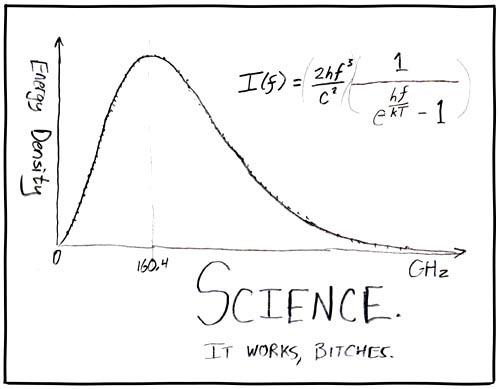
\includegraphics[width=0.7\linewidth]{./science}\\

\href{http://xkcd.com/54/}{XKCD}
\end{center}

\end{frame}

\end{document}